%
%  version 1, 2016-12-05
%
\documentclass[twocolumn,twoside]{svmultivs_br} %please do not change this line
\usepackage{graphicx}
\usepackage{tabularx}

\title*{Norwegian Mapping Authority Analysis Center Biennial Report}
\subtitle{2023--2024}
\titlerunning{NMA AC 2023--2024}

%\author{Name of First Author$^1$, Name of Second Author$^{1,2}$, Name of Third Author$^3$}
%\authorrunning{Last Name(s) of Author(s)} % see comments below
%\authoremails{e-mail address of first author, e-mail address of second author, e-mail address of third author}
%\institute{1. Institution Name 1 \\ 2. Institution Name 2 \\ 3. Institution Name 3}

\author{Ann-Silje Kirkvik}
\authorrunning{Kirkvik} % see comments below
\authoremails{ann-silje.kirkvik@kartverket.no}
\institute{Norwegian Mapping Authority (NMA)}

\component{NMA Analysis Center} 

\ContactAuthorName{Ann-Silje Kirkvik}
\ContactAuthorTelephone{+47 32118421}
\ContactAuthorEmail{ann-silje.kirkvik@kartverket.no}

\NumberofInstitutions{1}
\InstitutionPostAddress{1}{Postboks 600 Sentrum, 3507 H\onefoss}
\InstitutionCountry{1}{Norway}
\InstitutionWebPage{1}{https://www.kartverket.no}


\begin{document}  %please do not change this line
%
\maketitle       %please do not change this line
%
\abstract{During 2023 and 2024, the Norwegian Mapping Authority analysis center has contributed to the ITRF2020 
update (ITRF2020-u2023) and the operational daily SINEX product using the analysis software \textbf{Where}. NMA
has also participated in the IVS Working group on VLBI scale (WG9) and the 
analysis center continues to  
investigate the performance of the VLBI stations in Ny-\AA lesund. If the NMA gets funding
through the ESA program PRODEX, \textbf{Where} will be further developed to support VLBI observations of the Genesis satellite.}
%
\section{General Information}
%
The Norwegian Mapping Authority (NMA) has been an Associate Analysis Center
within the IVS since 2010. The analysis center is operated by the Geodetic
Institute at NMA with the headquarter in H\o nefoss, Norway. NMA is a governmental
agency with approximately 750 employees and the IVS activities at NMA are so far
completely funded by the Norwegian government.

NMA is using the analysis software \textbf{Where}, which is developed at NMA.
\textbf{Where}\footnote{https://kartverket.github.io/where} and its companion 
library \textbf{Midgard} \footnote{https://kartverket.github.io/midgard} is
freely available as open source at GitHub.

\textbf{Where} is at the moment capable of analyzing single sessions of VLBI data. 
Some scripts are also provided to investigate the results of the single session analysis.

\subsection{Staff}
The Geodetic Institute at NMA is lead by Per Erik Opseth and has approximately 50 employees. Some of its 
responsibilities include maintaining the
national reference frame, geoid and height system. The Geodetic Institute also provides a network-RTK positioning
service and operates the VLBI stations in Ny-\AA lesund \cite{ivsgm2022-nyal}.

In 2023 and 2024 the analysis center belonged to a team centered around global reference frames. Among the members
were Halfdan Pascal Kierulf working on reference frames and national and regional land uplift models and Laila L\o vh\o iden
working towards the establishment of the UN-Global Geodetic Center of Excellence (UN-GGCE). This team also
included the station leader in Ny-\AA lesund, Susana Garcia-Espada, and Leif Morten Tangen assisting with the operations in
Ny-\AA lesund from the main office in H\o nefoss. Ole Johan Klingan, who is working to acquire the new 
SLR instrument that will be installed in Ny-\AA lesund, was the team leader in this period. The daily activities of the analysis center were operated by a small group
consisting of one software developer and three part time analysts (see table \ref{tab:staff}).

\begin{table}[htb!]
\caption{NMA Analysis Center staff}
\begin{center}
\begin{tabularx}{\linewidth}{X|X}
\hline
Name  & Role \\
\hline
Ann-Silje Kirkvik & Developer and analyst \\
\AA smund Skj\ae veland & Analyst \\
Hans Sverre Smal\o & Analyst \\
\hline
\end{tabularx}
\end{center}
\label{tab:staff}
\end{table}
%
\section{Activities during the Past Year}
The activity level for the NMA analysis center has been reduced in the years 2023 and 2024 due to lack 
of resources. The analysis center has maintained the submission of the daily SINEX product and contributed
to the updated ITRF2020. The development of \textbf{Where} has been reduced to a minimum in this period. 
Halfdan Pascal Kierulf is participating in the IVS Working Group on VLBI Scale (WG9) and some additional data 
analysis have been performed to investigate and monitor Ny-\AA lesund specifically.

\subsection{IVS Working Group on VLBI Scale}
In the previous period, NMA participated in the IVS task force on scale \cite{biennial-acnma2021} with two members. When
the task force was formally changed to a working group NMA joined with one member. In this working group NMA has studied
the non-linear uplift due to glacial loading in Arctic areas. The effect on the VLBI station in Ny-Ålesund is considerable. 
Due to the non-linear nature of this uplift it can map into other reference parameters and explain parts of the VLBI-scale 
drift in ITRF2020. The work was presented at EGU2024.

\subsection{Daily SINEX and ITRF2020 updates}
Since 2019 NMA has submitted processed VLBI sessions routinely in the form of normal equations in the SINEX
format (Solution INdependent EXchange format). This is an analysis product that provides estimates of Earth 
orientation and site positions for each 24-hour session. For the rapid sessions R1 and R4, a timely turnaround 
of 14 days from observation to final product is desired. These sessions provide up to date Earth Orientation 
Parameters (EOP) to the global community. The contribution from NMA is included in the IVS combined solution.

In addition to processing R1 and R4 sessions, the analysis center also processes and submits SINEX files for 
most 24 sessions. When ITRF2020 was released, the entire VLBI history was reprocessed and this is the latest solution
that is currently being updated. The submitted solutions can be found at the IVS
Data Centers with the solution code \texttt{2023a}.

There is also a second solution named \texttt{2023b} which
is identical to \texttt{2023a} except it does not contain corrections for non tidal atmospheric loading. This solution
is used for ITRF2020 updates and is updated annually when a new ITRF2020 update is planned. 

\subsection{Ny-\AA lesund}
In February 2020, the new VLBI station NYALE13S had its first successful 24 hour session with a tri-band receiver. 
Since then, the baseline NYALE13S-NYALES20 have been monitored to investigate performance of the new station 
\cite{biennial-acnma2021}. In September 2023, the NYALES20 antenna was dismantled and this baseline will no longer 
be updated with new data \cite{biennial-stanma2023}. When more sessions with both the NYALE13S and NYALE13N antenna
recording together are available the monitoring of a local baseline in Ny-Ålesund can continue. In this case it will be useful to 
compare with other local baselines with two VGOS receivers.

At the general meeting in Tsukuba in 2024 the question was raised about the elevation mask
used at the NYALE13S (and NYALE13N) antenna(s). The elevation mask is set to 15 degrees to avoid destroying the Low Noise
Amplifiers (LNA) when boats with radar are in the harbor. The question is whether this high elevation mask degrades 
the solution and specifically the height component of the station coordinate. Some efforts have been made to investigate this, 
but more work is needed. The risk of destroying the LNAs is prohibiting the collection of data with lower elevation for comparison. 
There are however a few sessions from 2020 with some observations below 15 degrees. This was not intended, but luckily 
there was very little cruise traffic in Ny-\AA lesund during the COVID-19 pandemic and the amplifiers were not destroyed.

The baseline length repeatability of the NYALE13S-NYALES20 baseline is higher than the comparable baseline WETTZELL-WETTZ13N.
The reason for this is unknown, but preliminary analysis shows that the baseline length repeatability is degraded more by
removing all lower elevation angle observations than when removing a similar number of observations at random elevation angles.
See table \ref{tab:baselines}. Can the high elevation mask explain some of the higher baseline length repeatability in Ny-\AA lesund?

\begin{table}[t]
%\captionsetup{labelfont={color=black}}
	\begin{tabularx}{\linewidth}{X|l|r|r|r}
	Baseline & Scenario & WBL & WBLR & dL \\
	\hline
	Ns-Ny & no discard  & ~1539.1940 m & ~5.22 mm &  ~0.88 mm \\
	Ns-Ny & {15$^\circ$} elevation & ~1539.1944 m & ~6.42 mm &  ~1.26 mm \\
	Ns-Ny & random       & ~1539.1941 m & ~5.44 mm &  ~1.02 mm \\
	\hline
	Wz-Wn & no discard  &  ~123.3069 m & ~2.81 mm & ~-0.14 mm \\
	Wz-Wn & {15$^\circ$} elevation &  ~123.3064 m & ~3.66 mm & ~-0.58 mm \\
	Wz-Wn & random       &  ~123.3069 m & ~2.73 mm & ~-0.10 mm \\
	\hline
	\end{tabularx}
\caption{{Weighted baseline length (WBL), weighted baseline length repeatability (WBLR) and the difference 
between weighted baseline length and local tie vector (dL) for the different baselines. The second column describes which
criteria that has been used to discard observations (for all stations in the session). Ns-Ny is the NYALE13S-NYALES20 
baseline and Wz-Wn is the WETTZELL-WETTZ13N baseline. The number of observations discarded is the same for the 15 degrees
and random scenarios.
}}
\label{tab:baselines}
\end{table}

%
\section{Current Status}
%
Currently, the analysis center is preparing a submission for the next ITRF2020 update (ITRF2020-u2024). Contributions to the
regular daily SINEX product continue as normal. The daily SINEX product will switch to a new solution using the ITRF2020-u2023 
as a priori when the IVS agrees upon a date to perform the switch. The IVS also needs to decide how many old sessions that should
be reprocessed for each yearly ITRF update. 
%
\section{Future Plans}
%
NMA is in a process to apply for funding through the ESA program PRODEX. If the application is accepted part of the funding
will be used to continue the development of \textbf{Where}. Specifically, functionality will be added to \textbf{Where} to
enable processing of VLBI sessions tracking the Genesis satellite \footnote{https://www.esa.int/Applications/Satellite\_navigation/Genesis}.
%
% Code to include a single column figure through \includegraphics.
% \begin{figure} and \end{figure} make this single column.
% If the figure is too wide, it will overwrite text in the other column.
% Figures should be centered through the latex \begin{center} and
% \end{center} commands.  
% Captions should be left-justified.  
% The class file will automatically perform the left-justification,
% if the caption is not included in the latex centering.
%
%\begin{figure}[htb!]         
%  \begin{center}
%
% Please specify the file extension as part of the figure
% file name. The formats of jpg, png and pdf can be used.
% Sample files names are: 
%       acgsfc01.jpg  
%       tdgsfc01.png and tdgsfc02.png
%       occore01.jpg, occore02.png, and occore03.pdf.
%
%  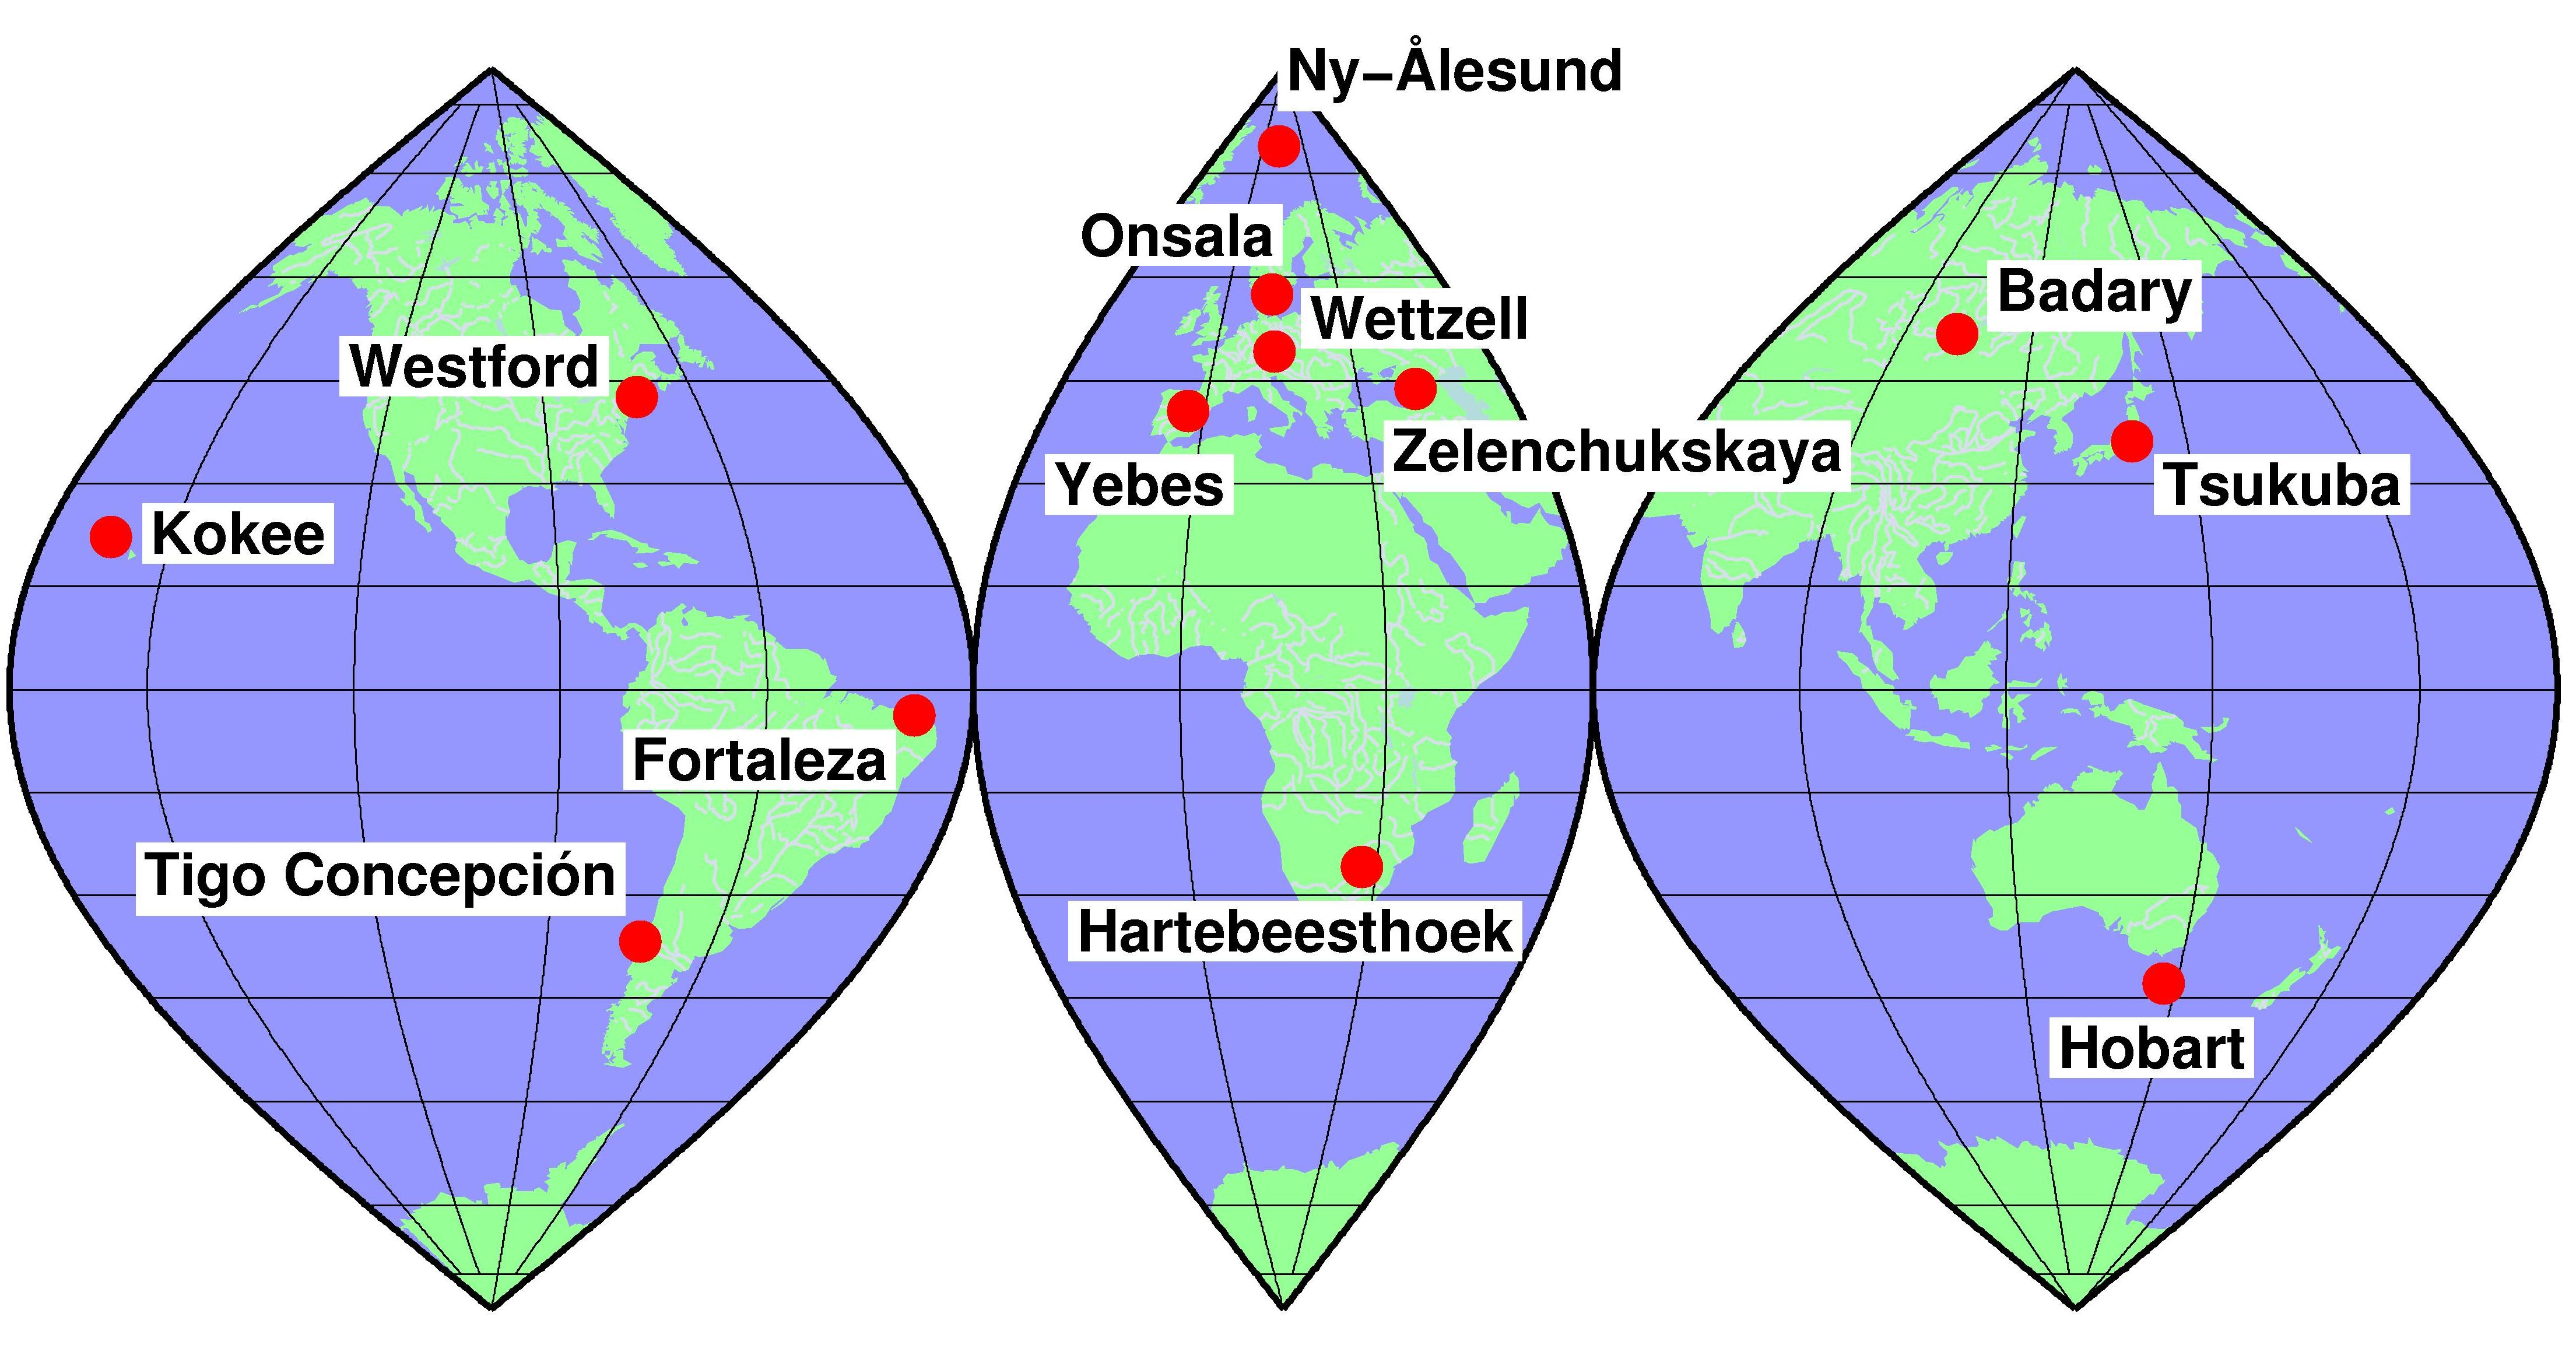
\includegraphics[width=.5\textwidth]{ivs-br-template01.jpg}
%%%%%  The caption should not be preceded by Figure 1.  
%%%%%  Please just enter your desired caption, such as:
%%%%%         Equipment at our station.
%  \end{center}
%  \caption{Example of figure from .jpg file.}
%  \label{first-unique-label}             
%\end{figure}                     
%
% Code to use \includegraphics to include a figure that spans two columns. 
% \begin{figure*} and \end{figure*} will allow the figure to Span 
% two columns.  If the figure is too narrow, it will leave blank space 
% in the other column.
% Figures should be centered through the latex \begin{center} and
% \end{center} commands.  
% Captions should be left-justified.  
% The class file will automatically perform the left-justification,
% if the caption is not included in the latex centering.
%
%\begin{figure*}[htb!]
% Please see the above figure example for naming conventions for the 
% figure file.
%\begin{center}
%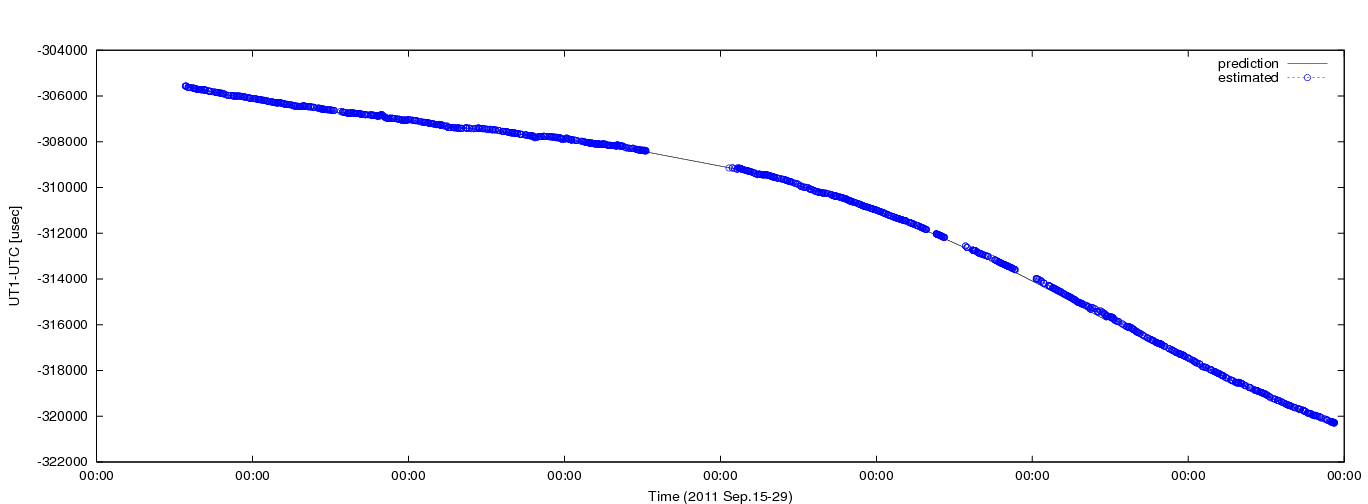
\includegraphics[width=16.0cm]{ivs-br-template02.png}
%\end{center}
% Please do not precede the caption by Figure 2.  
% Please just enter your desired text.
%\caption{Example of figure from .png file.}
%\label{second-unique-label}
%\end{figure*}
%
% Code to include a single column table.
% Other table formats may be used also.  
% Tables should be centered through the latex \begin{center} and
% \end{center} commands.  
% Captions should be left-justified.  
% The class file will automatically perform the left-justification,
% if the caption is not included in the latex centering.
%
%\begin{table}[htb!]
%\caption{Caption for Table 1.}
%\begin{center}
%\begin{tabular}{|l|c|c|r|} \hline
%Heading 1 & Heading 2 & Heading 3 & Heading 4\\
%\hline
%Value a1 & Value a2 & Value a3 &          \\
%Value b1 &          & Value b3 & Value b4 \\
%Value c1 & Value c2 & Value c3 &          \\
%Value d1 & Value d2 & Value d3 & Value d4 \\
%Value e1 & Value e2 & Value e3 & Value e4 \\
%\hline
%\end{tabular}
%\end{center}
%\label{third-unique-label}
%\end{table}
%
% Code to include a two column table.
% Other table formats may be used also.  
% Tables should be centered through the latex \begin{center} and
% \end{center} commands.  
% Captions should be left-justified.  
% The class file will automatically perform the left-justification,
% if the caption is not included in the latex centering.
%
%\begin{table*}[htb!]
%\caption{Caption for Table 2.}
%\begin{center}
%\begin{tabular}{|l|c|c|r|l|c|c|r|} \hline
%Heading 1 & Heading 2 & Heading 3 & Heading 4 & Heading 5 & Heading 6 & Heading 7 & Heading 8\\
%\hline
%Value a1 & Value a2 & Value a3 &          & Value a5 & Value a6 & Value a7 & Value a8 \\
%Value b1 &          & Value b3 & Value b4 &          &          & Value b7 & Value b8 \\
%Value c1 & Value c2 & Value c3 &          & Value c5 & Value c6 & Value c7 &          \\
%Value d1 & Value d2 & Value d3 & Value d4 & Value d5 & Value d6 &          &          \\
%Value e1 & Value e2 & Value e3 & Value e4 & Value e5 &          & Value e7 &          \\
%Value f1 & Value f2 & Value f3 & Value f4 & Value f5 &          & Value f7 &          \\
%V%alue g1 &          & Value g3 & Value g4 & Value g5 & Value g6 & Value g7 & Value g8 \\
%%\hline
%Value h1 & Value h2 & Value h3 &          & Value h5 & Value h6 & Value h7 & Value h8 \\
%Value i1 &          & Value i3 & Value i4 &          &          & Value i7 & Value i8 \\
%Value j1 & Value j2 & Value j3 &          & Value j5 & Value j6 & Value j7 &          \\
%Value k1 & Value k2 & Value k3 & Value k4 & Value k5 & Value k6 &          &          \\
%Value l1 & Value l2 & Value l3 & Value l4 & Value l5 &          & Value l7 &          \\
%Value m1 & Value m2 & Value m3 & Value m4 & Value m5 &          & Value m7 &          \\
%%Value n1 &          & Value n3 & Value n4 & Value n5 & Value n6 & Value n7 & Value n8 \\
%\hline
%%Value o1 & Value o2 & Value o3 &          & Value o5 & Value o6 & Value o7 & Value o8 \\
%%Value p1 &          & Value p3 & Value p4 &          &          & Value p7 & Value p8 \\%v
%%%%%V%%alue q1 & Value q2 & Value q3 &          & Value q5 & Value q6 & Value %q7 &          \\
%Value r1 & Value r2 & Value r3 & Value r4 & Value r5 & Value r6 &          &          \\
%%%%%%Value s1 & Value s2 & Value s3 & Value s4 & Value s5 &          & Value s7 &          \\
%Value t1 & Value t2 & Value t3 & Value t4 & Value t5 &          & Value t7 &          \\%v
%%Value u1 &          & Value u3 & Value u4 & Value u5 & Value u6 & Value u7 & Value u8 \\
%\hline
%%Value v1 & Value v2 & Value v3 &          & Value v5 & Value v6 & Value v7 & Value v8 \\
%%%Value w1 &          & Value w3 & Value w4 &          &          & Value w7 & Value w8 \\
%%Value x1 & Value x2 & Value x3 &          & Value x5 & Value x6 & Value x7 &          \\
%Value y1 & Value y2 & Value y3 & Value y4 & Value y5 & Value y6 &          &          \\
%Value z1 & Value z2 & Value z3 & Value z4 & Value z5 &          & Value z7 &          \\
%\hline
%\end{tabular}
%\end{center}
%\label{fourth-unique-label}
%\end{table*}
%
% Please see the first two figures for detailed information
% about using figures.
%
%\begin{figure*}[htb!]
%\begin{center}
%\includegraphics[width=16.0cm]{ivs-br-template03.pdf}
%\end{center}
%\caption{Example of figure from .pdf file.}
%\label{fifth-unique-label}
%\end{figure*}
%
% The acknowledgements section is optional.  If used, the section line should 
% be:
%      \section*{Acknowledgements}
%
%\section*{Acknowledgements}

%This section is optional.
%
% The bibliography section is optional.
%
% Here is a section with some examples.
% But the entries are free-format --- essentially,
%  \bibitem{unique-label}
%  text
%
%%%%%\begin{thebibliography}{99}
%%%%%\bibitem{Abbondanza2012}
%%%%%C.~Abbondanza and P.~Sarti.
%%%%%Impact of network geometry, observation schemes and telescope structure deformations on local ties:
%%%%%simulations applied to Sardinia Radio Telescope.
%%%%%\emph{Journal of Geodesy}, 86(3), doi:10.1007/s00190-011-0507-6, 181--192, 2012.
%%
%%%%%\bibitem{Artz}
%%%%%Thomas Artz, Judith Leek, Axel Nothnagel, and Maike Schumacher.
%%%%%VLBI Intensive Sessions Revisited.
%%%%%In D.~Behrend and K.~Baver, editors, \emph{International
%%%%%  VLBI Service for Geodesy and Astrometry 2012 General Meeting Proceedings},
%%%%%  NASA/CP-2012-217504, pages 276--280, 2012.
%%%%%%%
%%%%%\bibitem{VieVS}
%%%%%Matthias Madzak, Sigrid B\"ohm, Hana Kr\'asn\'a, and Lucia Plank.
%%%%%Vienna VLBI Software Version 2.1 User Manual
%%%%%Web document http://vievs.geo.tuwien.ac.at/fileadmin/editors/VieVS/documents/vievsDoc.pdf
%%%%%%
%%%%%\end{thebibliography}
\begin{thebibliography}{99}

\bibitem{ivsgm2022-nyal}
Susana Garcia-Espada et al. ``Status at Ny-Ålesund Geodetic Earth Observatory'',
In IVS 2022 General Meeting Proceedings, edited by K.\ Armstrong, D.\ Behrend, and K.\ Baver,
NASA/CP-20220018789, 2023
\bibitem{biennial-acnma2021}
Ann-Silje Kirkvik, ``Norwegian Mapping Authority Analysis Center Biennial Report 2021--2022'',
In International VLBI Service for Geodesy and Astrometry 2021+2022 Biennial Report, 
edited by K. L. Armstrong, D. Behrend, and K. D. Baver, NASA/TP-20230014975, 2023.
\bibitem{biennial-stanma2023}
Susana Garcia-Espada et al., ``Ny-\AA lesund Geodetic Observatory'', 
In International VLBI Service for Geodesy and Astrometry 2023+2024 Biennial Report,
this volume.
%\bibitem{IVS-CC}
%D.~Behrend, ``Coordinating Center Report'',
%In K.\ D.\ Baver, D.\ Behrend, and K.\ Armstrong, editors, International
%VLBI Service for Geodesy and Astrometry 2012 Annual Report,
%NASA/TP-2013-217511, pages 55--57, 2013.

\end{thebibliography}
%
\end{document}
